Ở chương trước, chúng tôi đã trình bày những khảo sát về các công trình liên quan tới nghiên cứu của chúng tôi. Từ đó, trong chương này, chúng tôi sẽ đề xuất một mô hình giải pháp cho bài toán phát hiện và phòng thủ trước tấn công DoS/DDoS dựa trên mục tiêu và hướng tiếp cận vấn đề mà chúng tôi đã nêu ra ở Chương Giới thiệu.

\section{Tập dữ liệu dùng để huấn luyện: CICIDS2018}
\label{ids-dataset}

CSE-CIC-IDS2018 (gọi tắt CICIDS2018) \cite{36a-ids2018} là dataset bao gồm nhiều loại tấn công giúp xây dựng hệ thống phát hiện xâm nhập. Đây là dự án kết hợp giữa Communications Security Establishment (CSE) \& the Canadian Institute for Cybersecurity (CIC). Theo báo cáo, để thực hiện tạo dựng dataset này, tác giả đã xậy dựng 7 hệ thống mạng với 500 máy tính trên nền tảng AWS. Mô hình mạng này được biểu thị trong hình \ref{fig:aws-ids2018}.

\begin{figure}[ht!]
	\centering
	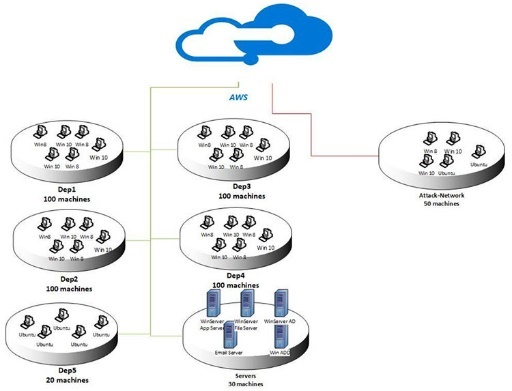
\includegraphics[width=0.75\linewidth]{fig/aws-ids2018.png}
	\caption{Mô hình mạng trong CSE-CIC-IDS2018}
	\label{fig:aws-ids2018}
\end{figure}

Các loại tấn công có trong dataset này bao gồm tấn công brute-force, tấn công heartbleed, Botnet, tấn công DoS, tấn công DDoS, tấn công Web, xâm nhập mạng từ bên trong.

Dataset được chia thành hai loại, thứ nhất là tập các tệp PCAP ghi nhận lưu lượng mạng và các mô tả về IP nguồn, IP đích và Protocol của các luồng tấn công và luồng hợp lệ, thứ hai là tập các tệp CSV được sinh ra từ phần mềm CICFlowMeter \cite{37-cicflowmeter} kèm với nhãn của các luồng đã được đánh dấu sẵn.

Do kích thước của các tệp PCAP rất lớn (lên tới hàng chục GB), nên trong khuôn khổ của khóa luận này, tôi sử dụng các tệp CSV đã được tạo sẵn với kích thước nhỏ hơn rất nhiều.

Dataset được chia ra thành từng ngày, mỗi ngày sẽ có một số loại tấn công được triển khai. Vì vậy, tôi chỉ chọn ra những ngày có tấn công DoS/DDoS được triển khai.

Danh sách các ngày được chọn trong bảng \ref{tab:day-choice-ids2018}.

\begin{table}[ht!]
\centering
	\begin{tabular}{|l|l|}
		\hline
		\multicolumn{1}{|c|}{\textbf{Ngày}} & \multicolumn{1}{c|}{\textbf{Mô tả}}                                                  \\ \hline
		Thurs-15-02-2018 & \begin{tabular}[c]{@{}l@{}}DoS-GoldenEye       \\    \\ DoS-Slowloris\end{tabular}   \\ \hline
		Fri-16-02-2018                      & \begin{tabular}[c]{@{}l@{}}DoS-SlowHTTPTest\\    \\ DoS-Hulk\end{tabular}   \\ \hline
		Tues-20-02-2018  & \begin{tabular}[c]{@{}l@{}}DDoS attacks-LOIC-HTTP\\    \\ DDoS-LOIC-UDP\end{tabular} \\ \hline
		Wed-21-02-2018                      & \begin{tabular}[c]{@{}l@{}}DDOS-LOIC-UDP    \\    \\ DDOS-HOIC\end{tabular} \\ \hline
	\end{tabular}
\caption{Danh sách các ngày được chọn trong dataset CICIDS2018}
\label{tab:day-choice-ids2018}
\end{table}

\subsection{Tiền xử lý và thống kê dữ liệu}
\label{preprocessing-data}

\subsubsection{Tiền xử lý}

Dữ liệu trong dataset không thật sự hoàn hảo, lý do đến từ phần CICFlowMeter vẫn còn một vài lỗi dẫn đến xuất hiện một số bản ghi trong dữ liệu chứa giá trị vô cực (Inf) hoặc không phải số (NaN). Vì vậy, bước cần thiết là loại bỏ các bản ghi lỗi này ra khỏi dataset.

Giải thuật tiền xử lý dữ liệu được mô tả trong lưu đồ \ref{fig:drop-line}.

\begin{figure}[ht!]
	\centering
	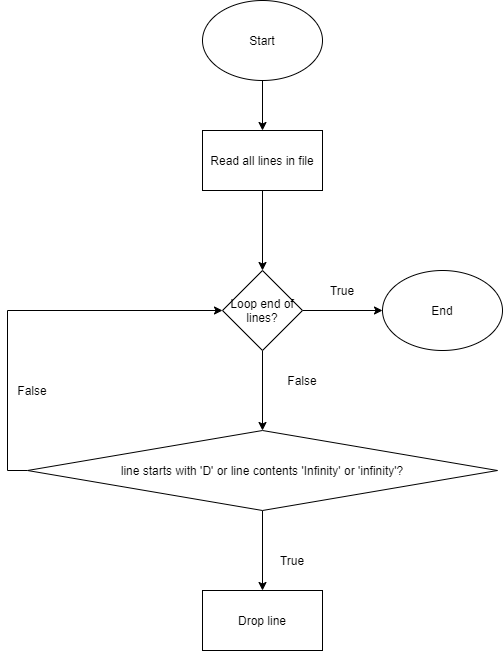
\includegraphics[width=0.75\linewidth]{fig/drop-line.png}
	\caption{Lưu đồ giải thuật tiền xử lý dataset}
	\label{fig:drop-line}
\end{figure}

\subsubsection{Thống kê}

Sau khi tiền xử lý dữa liệu, số lượng luồng hợp lệ và tấn công còn lại được ghi trong bảng \ref{tab:stat-ids2018}.

\begin{table}[ht!]
\centering
	\begin{tabular}{|l|l|l|}
		\hline
		\multicolumn{1}{|c|}{\textbf{Ngày}} & \multicolumn{1}{c|}{\textbf{Số luồng hợp lệ}} & \multicolumn{1}{c|}{\textbf{Số luồng tấn công}} \\ \hline
		Thurs-15-02-2018 & 987,980   & 52,498  \\ \hline
		Fri-16-02-2018   & 446,772   & 601,802 \\ \hline
		Tues-20-02-2018  & 7,313,104 & 576,191 \\ \hline
		Wed-21-02-2018   & 360,833   & 687,742 \\ \hline
	\end{tabular}
\caption{Bảng thống kê dữ liệu trong CICIDS2018}
\label{tab:stat-ids2018}
\end{table}

\subsection{Xử lý dữ liệu}

\subsubsection{Phân chia dữ liệu thành các tập con}

Vì mỗi một ngày chứa lưu lượng của một loại tấn công khác nhau, nên trước khi gộp dữ liệu các ngày lại với nhau, tôi tiến hành phân chia dữ liệu trên từng ngày thành 2 tập là tập huấn luyện và tập kiểm tra với tỷ lệ 8:2. Sau đó, tôi ghép các tập con này lại và thu được dataset đặt tên là \textbf{IDS-train} tương ứng với tập huấn luyện và \textbf{IDS-test} tương ứng với tập kiểm tra được thống kê trong bảng \ref{tab:sub-dataset}. Trước khi ghép các dữ liệu lại với nhau, tôi đã loại bỏ trường "Timestamp", vì trường này không quan trọng cho việc phân tích và huấn luyện.

\begin{table}[ht!]
\centering
	\begin{tabular}{|l|l|l|}
		\hline
		\multicolumn{1}{|c|}{\textbf{Tập}} & \multicolumn{1}{c|}{\textbf{Số luồng hợp lệ}} & \multicolumn{1}{c|}{\textbf{Số luồng tấn công}} \\ \hline
		IDS-train                          & 7,287,007                                     & 1,534,586                                       \\ \hline
		IDS-test                           & 1,821,682                                     & 383,647                                         \\ \hline
	\end{tabular}
\caption{Các tập dữ liệu con sau khi phân chia}
\label{tab:sub-dataset}
\end{table}

\subsubsection{Phân tích, tối ưu hóa dữ liệu}

Sau khi đã có dataset cuối cùng, tôi tiến hành phân tích và tối ưu dữ liệu để phục vụ cho việc huấn luyện.

\textit{Phân tích}

Tổng số đặc trưng mà CICFlowMeter trích xuất là 84, tuy nhiên khi tác giả công bố dataset đã bỏ đi một vài đặc trưng như Source IP, Source Port, Dest IP, vv, và thêm một đặc trưng được tôi loại bỏ là ''Timestamp'' nên tổng số đặc trưng còn lại là 78. Chi tiết các đặc trưng này trong bảng \ref{tab:feature-list}.

\begin{center}
	\centering
	\begin{longtable}{|l|l|l|}
		\hline
		\multicolumn{1}{|c|}{\textbf{STT}} & \multicolumn{1}{c|}{\textbf{Đặc trưng}} & \multicolumn{1}{c|}{\textbf{Mô tả}} \\ \hline
		1  & Dst Port          & Cổng   của địa chỉ IP đích trong gói tin IP        \\ \hline
		2  & Protocol          & Giao   thức mạng với 6 là TCP, 17 là UDP           \\ \hline
		3  & Flow Duration     & Tổng   thời gian của luồng                         \\ \hline
		4  & Tot Fwd Pkts      & Tổng   số gói tin trong luồng theo chiều tới (fwd) \\ \hline
		5  & Tot Bwd Pkts      & Tổng   số gói tin trong luồng theo chiều lui (bwd) \\ \hline
		6  & TotLen Fwd Pkts   & Tổng   độ dài của các gói tin fwd                  \\ \hline
		7  & TotLen Bwd Pkts   & Tổng   độ dài của các gói tin bwđ                  \\ \hline
		8  & Fwd Pkt Len Max   & Độ   dài max gói tin fwd                           \\ \hline
		9  & Fwd Pkt Len Min   & Độ   dài min gói tin fwd                           \\ \hline
		10 & Fwd Pkt Len Mean  & Mean   độ dài gói tin fwd                          \\ \hline
		11 & Fwd Pkt Len Std   & Độ   lệch chuẩn độ dài gói tin fwd                 \\ \hline
		12 & Bwd Pkt Len Max   & Độ   dài max gói tin bwd                           \\ \hline
		13 & Bwd Pkt Len Min   & Độ   dài min gói tin bwd                           \\ \hline
		14 & Bwd Pkt Len Mean  & Mean   độ dài gói tin bwd                          \\ \hline
		15 & Bwd Pkt Len Std   & Độ   lệch chuẩn độ dài gói tin bwd                 \\ \hline
		16 & Flow Byts/s       & Tổng   số bytes trong luồng / giây                 \\ \hline
		17 & Flow Pkts/s       & Tổng   số gói tinn trong luồng / giây              \\ \hline
		18 & Flow IAT Mean     & Mean   IAT luồng                                   \\ \hline
		19 & Flow IAT Std      & Độ   lệch chuẩn IAT luồng                          \\ \hline
		20 & Flow IAT Max      & Max   IAT luồng                                    \\ \hline
		21 & Flow IAT Min      & Min   IAT luồng                                    \\ \hline
		22 & Fwd IAT Tot       & Tổng   số IAT fwd                                  \\ \hline
		23 & Fwd IAT Mean      & Mean   IAT fwd                                     \\ \hline
		24 & Fwd IAT Std       & Độ   lệch chuẩn IAT fwd                            \\ \hline
		25 & Fwd IAT Max       & Max   IAT fwd                                      \\ \hline
		26 & Fwd IAT Min       & Min   IAT fwd                                      \\ \hline
		27 & Bwd IAT Tot       & Tổng   số IAT bwd                                  \\ \hline
		28 & Bwd IAT Mean      & Mean   IAT bwd                                     \\ \hline
		29 & Bwd IAT Std       & Độ   lệch chuẩn IAT bwd                            \\ \hline
		30 & Bwd IAT Max       & Max   IAT bwd                                      \\ \hline
		31 & Bwd IAT Min       & Min   IAT bwd                                      \\ \hline
		32 & Fwd PSH Flags     & Tổng   số cờ PSH fwd                               \\ \hline
		33 & Bwd PSH Flags     & Tổng   số cờ PSH bwd                               \\ \hline
		34 & Fwd URG Flags     & Tổng   số cờ URG fwd                               \\ \hline
		35 & Bwd URG Flags     & Tổng   số cờ URG bwd                               \\ \hline
		36 & Fwd Header Len    & Tổng   độ dài header các gói tin fwd               \\ \hline
		37 & Bwd Header Len    & Tổng   độ dài header các gói tin bwd               \\ \hline
		38 & Fwd Pkts/s        & Tổng   số gói tin fwd / giây                       \\ \hline
		39 & Bwd Pkts/s        & Tổng   số gói tin bwd / giây                       \\ \hline
		40 & Pkt Len Min       & Độ   dài min gói tin trong luồng                   \\ \hline
		41 & Pkt Len Max       & Độ   dài max gói tin trong luồng                   \\ \hline
		42 & Pkt Len Mean      & Độ   dài mean gói tin trong luồng                  \\ \hline
		43 & Pkt Len Std       & Độ   lệch chuẩn độ dài gói tin trong luồng         \\ \hline
		44 & Pkt Len Var       & Phương   sai độ dài gói tin trong luồng            \\ \hline
		45 & FIN Flag Cnt      & Tổng   số cờ FIN                                   \\ \hline
		46 & SYN Flag Cnt      & Tổng   số cờ SYN                                   \\ \hline
		47 & RST Flag Cnt      & Tổng   số cờ RST                                   \\ \hline
		48 & PSH Flag Cnt      & Tổng   số cờ PSH                                   \\ \hline
		49 & ACK Flag Cnt      & Tổng   số cờ ACK                                   \\ \hline
		50 & URG Flag Cnt      & Tổng   số cờ URG                                   \\ \hline
		51 & CWE Flag Count    & Tổng   số cờ CWE                                   \\ \hline
		52 & ECE Flag Cnt      & Tổng   số cờ ECE                                   \\ \hline
		53 & Down/Up Ratio     & Lưu   lượng fwd / lưu lượng bwd                    \\ \hline
		54 & Pkt Size Avg      & Kích   thước trung bình của gói tin                \\ \hline
		55 & Fwd Seg Size Avg  & Kích   thước trung bình gói tin fwd                \\ \hline
		56 & Bwd Seg Size Avg  & Kích   thước trung bình gói tin bwd                \\ \hline
		57 & Fwd Byts/b Avg    & Số   bytes/bulk trung bình fwd                     \\ \hline
		58 & Fwd Pkts/b Avg    & Số   gói tin/bulk trung bình fwd                   \\ \hline
		59 & Fwd Blk Rate Avg  & Tỷ   lệ bulk fwd trung bình                        \\ \hline
		60 & Bwd Byts/b Avg    & Số   bytes/bulk bwd                                \\ \hline
		61 & Bwd Pkts/b Avg    & Số   gói tin/bulk bwd                              \\ \hline
		62 & Bwd Blk Rate Avg  & Tỷ   lệ bulk bwd trung bình                        \\ \hline
		63 & Subflow Fwd Pkts  & Số   gói tin trong luồng con fwd                   \\ \hline
		64 & Subflow Fwd Byts  & Số   bytes trong luồng con fwd                     \\ \hline
		65 & Subflow Bwd Pkts  & Số   gói tin trong luồng con bwd                   \\ \hline
		66 & Subflow Bwd Byts  & Số   bytes trong luồng con  bwd                    \\ \hline
		67 & Init Fwd Win Byts & TCP   window size của gói tin đầu tiên fwd         \\ \hline
		68 & Init Bwd Win Byts & TCP   window size của gói tin đầu tin bwd          \\ \hline
		69 & Fwd Act Data Pkts & Số   gói tin thật sự có payload fwd                \\ \hline
		70 & Fwd Seg Size Min  & Kích   thước header nhỏ nhất fwd                   \\ \hline
		71 & Active Mean       & Mean   thời gian active                            \\ \hline
		72 & Active Std        & Độ   lệch chuẩn thời gian active                   \\ \hline
		73 & Active Max        & Max   thời gian active                             \\ \hline
		74 & Active Min        & Min   thời gian active                             \\ \hline
		75 & Idle Mean         & Mean   thời gian idle                              \\ \hline
		76 & Idle Std          & Độ   lệch chuẩn thời gian idle                     \\ \hline
		77 & Idle Max          & Max   thời gian idle                               \\ \hline
		78 & Idle Min          & Min   thời gian idle                               \\ \hline
	\caption{Danh sách các đặc trưng của luồng gói tin được rút trích}
	\label{tab:feature-list}
	\end{longtable}
\end{center}

\textit{Tối ưu hóa}

Tôi sử dụng phương pháp Feature Selection với hàm ChiSquare để chọn ra các đặc trưng thật sự cần thiết cho việc huấn luyện.
Tôi sử dụng thư viện scikit-learn để thực hiện. Giải thuật được mô tả trong sơ đồ hình \ref{fig:feature-selection}.

\begin{figure}[ht!]
	\centering
	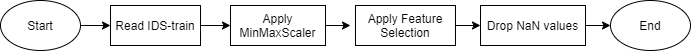
\includegraphics[width=\linewidth]{fig/feature-selection.png}
	\caption{Lưu đồ tối ưu hóa dataset}
	\label{fig:feature-selection}
\end{figure}

Từ đó tôi loại bỏ được 11 đặc trưng gồm Dst Port, Bwd PSH Flags, Fwd URG Flags, Bwd URG Flags, CWE Flag Count, Fwd Byts/b Avg, Fwd Pkts/b Avg, Fwd Blk Rate Avg, Bwd Byts/b Avg, Bwd Pkts/b Avg, Bwd Blk Rate Avg. Từ đó còn lại 67 đặc trưng cho việc huấn luyện.

\section{Các mô hình huấn luyện}

Trước khi áp dụng huấn luyện, tôi chuyển các giá trị âm trong dữ liệu thành 0, sau đó thực hiện normalize dữ liệu bằng hàm normalize trong thư viện Keras. Hàm này sử dụng L2 norm để normalize dữ liệu.

\subsection{Các chỉ số đánh giá mô hình}

Trong bài toán hiện tại tôi đang giải quyết là bài toán phân lớp nhị phân, vì vậy kết quả đầu ra là Positive (Attack) hay Negative (Benign).
Ma trận nhầm lẫn (Confusion matrix) của tôi sẽ có dạng như bảng \ref{tab:confusion_matrix_pattern}. Với TP, FP, TN, FN tương ứng với True Positive, False Positive, True Negative, False Negative.

\begin{table}[ht!]
\centering
	\begin{tabular}{|l|l|l|l|}
		\hline
		&                   & \textbf{Predicted} &                   \\ \hline
		&                   & \textit{Negative}  & \textit{Positive} \\ \hline
		\textbf{True} & \textit{Negative} & \# of TN           & \# of FP          \\ \hline
		& \textit{Positive} & \# of FN           & \# of TP          \\ \hline
	\end{tabular}
\caption{Mẫu ma trận nhầm lẫn}
\label{tab:confusion_matrix_pattern}
\end{table}

Khi đó, công thức của các chỉ số đánh giá như sau.

\textit{Accuracy}: 
\[ Acc = \frac{TP + TN}{Total} \]
\textit{Precision} (hay Positive predictive value):
\[ Pre = \frac{TP}{TP + FP} \]
\textit{Recall}:
\[ Rec = \frac{TP}{TP + FN} \]
\textit{F1-score}:
\[ F1 = 2 \frac{Pre \cdot Rec}{Pre + Rec} \]

\subsection{Mô hình học máy}

Trong phần này, tôi giới thiệu chi tiết các mô hình học máy gồm Support Vector Machine, Naïve Bayes, Decision Tree.

\subsubsection{Support Vector Machine}

Tham khảo từ nghiên cứu \cite{67-Patle} của A. Patle và cộng sự, SVM phân loại lớp bằng việc tạo ra một siêu phẳng (hyperplane) N chiều. SVM là một thực thể toán học, một giải thuật để tối đa hóa một hàm toán học cụ thể đối với một tập dữ liệu nhất định. SVM có 4 khái niệm cơ bản:

\begin{itemize} 
	\item[--] Siêu phẳng phân chia (Separating hyperplane)
	\item[--] Siêu phẳng biên cực đại (Maximum-margin hyperplane)
	\item[--] Biên mềm (Soft Margin)
	\item[--] Hàm cốt lõi (Kernel function)  
\end{itemize}
 
 \textit{Biên}
 
 Biên là khoảng cách giữa siêu phẳng đến hai điểm dữ liệu gần nhất tương ứng với các phân lớp.
 
 \textit{Siêu phẳng phân chia}
 
 Đường thẳng chia không gian thành 2 phần, và ở không gian ba chiều chúng ta cần mặt phẳng để phân chia không gian. Định nghĩa chung cho ranh giới phân chia trong không gian N chiều là siêu phẳng. Vì vậy, siêu phẳng phân chia là ranh giới về cơ bản phân chia các mẫu khác nhau trong tập dữ liệu. Hình \ref{fig:separating-hyperplane} ví dụ một siêu phẳng phân chia.
 
 \begin{figure}[ht!]
 	\centering
 	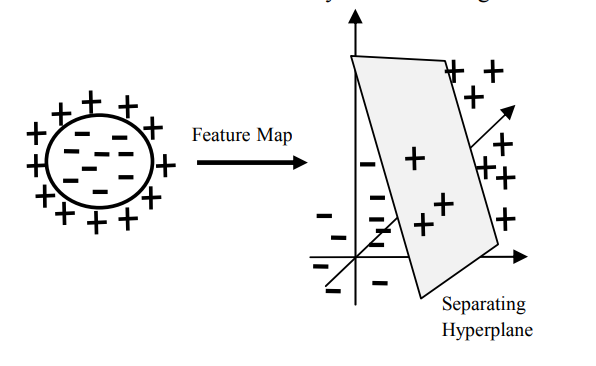
\includegraphics[width=0.5\linewidth]{fig/separating-hyperplane.png}
 	\caption{Ví dụ siêu phẳng phân chia}
 	\label{fig:separating-hyperplane}
 \end{figure}

\textit{Siêu phẳng biên cực đại (siêu phẳng tối ưu)}

Siêu phẳng biên cực đại nghĩa là lựa chọn ranh giới ở chính giữa. Nói cách khác, ranh giới được chọn để phân chia hai lớp phải đáp ứng được biên là lớn nhất.

Theo \cite{68-Vapnik}, cách giải thích của Vapnik và cộng sự trình bày về khái niệm này như sau. Ta có một tập huấn luyện được gán nhãn

\begin{gather}
	\label{svm:1}
	(y_1, x_1), ... , (y_l, x_l), y_i \in {-1, 1}
\end{gather}

được xem là có thể phân chia tuyến tính nếu tồn tại một vec-tơ \( \textbf{w} \) một đại lượng vô hướng \( \textit{b}\) sao cho các bất bất đẳng thức

\begin{equation}
	\begin{gathered}
	\label{svm:2}
		w \cdot x_i + \textit{b} \geq 1 \quad \quad \quad \quad if \quad \quad y_i = 1, \\
		w \cdot x_i + \textit{b} \leq 1 \quad \quad \quad \quad if \quad \quad y_i = -1
	\end{gathered}
\end{equation}

đều thỏa tất cả phần tử trong tập huấn luyện (\ref{svm:1}). Viết lại bất đẳng thức (\ref{svm:2})

\begin{gather}
	\label{svm:3}
	y_i (w \cdot x_i + \textit{b}) \geq 1, \quad \quad \quad i = 1, ..., l
\end{gather}

Siêu phẳng tối ưu

\begin{gather}
	\label{svm:4}
	w_0 \cdot x + \textit{b}_0 = 0
\end{gather}

là siêu phẳng duy nhất chia dữ liệu huấn luyện với biên lớn nhất: nó xác định hướng của \textbf{w}/|\textbf{w}| sao cho khoảng cách khoảng cách hình chiếu của vec-tơ huấn luyện của hai lớp khác nhau là tối đa.

\textit{Biên mềm}

SVM có thể chịu được lỗi trong dữ liệu bằng cách cho phép một vài dữ liệu bị phân lớp sai. Để làm được vậy, giải thuật SVM chỉnh sửa và thêm vào “biên mềm” (Hình \ref{fig:svm-soft-margin}). Cơ bản, điều này cho phép một số điểm dữ liệu di chuyển qua rìa của siêu phẳng phân chia mà không ảnh hưởng đến kết quả cuối cùng. Trong hình \ref{fig:svm-soft-margin}, siêu phẳng là B1 và B2. B1 tốt hơn B2 vì nó tối đa hóa biên. 

\begin{figure}[ht!]
	\centering
	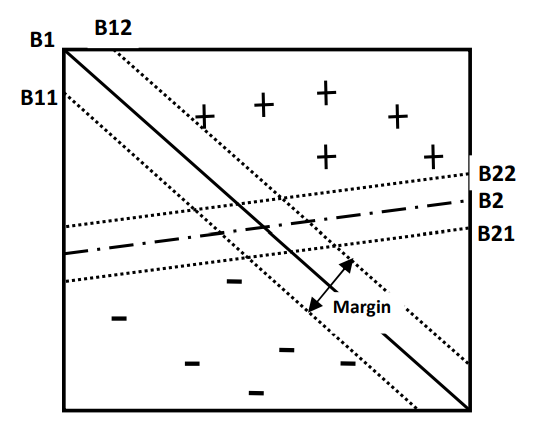
\includegraphics[width=0.5\linewidth]{fig/svm-soft-margin.png}
	\caption{Ví dụ biên mềm}
	\label{fig:svm-soft-margin}
\end{figure}

\textit{Hàm cốt lõi}

Hàm cốt lõi là thủ thuật toán học cho phép SVM phân lớp trong không gian hai chiều của một tập dữ liệu ở không gian một chiều. Nói chung, một hàm cốt lõi ánh xạ dữ liệu từ một không gian chiều thấp đến một không gian có chiều cao hơn. Công thức bên dưới và hình \ref{fig:svm-kernel} thể hiện cách hàm cốt lõi ánh xạ dữ liệu.

\[ \langle x_1 \cdot x_2 \rangle \leftarrow K(x_1,x_2) = \langle \Phi(x_1) \cdot \Phi(x_2) \rangle \]

 \begin{figure}[ht!]
 	\centering
	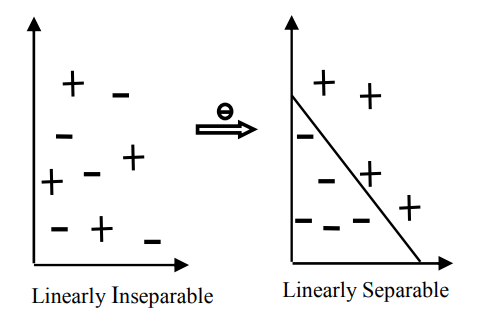
\includegraphics[width=0.5\linewidth]{fig/svm-kernel.png}
	\caption{Cách hàm cốt lõi ánh xạ dữ liệu}
	\label{fig:svm-kernel}
\end{figure}

\textit{Hàm cốt lõi tuyến tính (Linear Kernel Function)}

Hàm cốt lõi tuyến tính được biểu diễn như sau: \( K(x, x_j) = x \cdot x^T\)

\subsubsection{Naïve Bayes}

Theo nghiên cứu của Rish và các cộng sự \cite{71-Rish}, giải thuật phân lớp Naïve được diễn giải như sau.

Cho \( X = X_1, ..., X_n\) là một vec-tơ những biến ngẫn nhiên, được gọi là đặc trưng, với mỗi đặc tính lấy giá trị tiền miền $D_i$ của nó. Tập tất cả các vec-tơ đặc trưng được ký hiệu  \(\Omega = D_1 \times ... \times D_n\). Cho $C$ là một biến ngẫu nhiên không quan sát ký hiệu cho phân lớp của mẫu, $C$ có thể giữa một giá trị trong $m$ giá trị $c \in {0,...,m-1}$.

Một hàm \(g: \Omega \rightarrow {0,...,m-1}\), với $g(x) = C$ ký hiệu một \textit{khái niệm} được học. 

Một  máy phân lớp được định nghĩa bởi một hàm $h: \Omega \rightarrow {0,...,m-1}$ (một hypothesis) gán một lớp cho bất cứ mẫu được cho nào. Một hướng tiếp cận thông dụng là liên kết mỗi lớp $i$ với một hàm phân biệt \( f_i(X), i={0,...,m-1}\), và để cho máy phân lớp chọn phân lớp với hàm phân biệt lớn nhất trên một mẫu được cho: \(h(x)  = argmax_{i \in {0,...,m-1}f_i(x)}\).

Máy phân lớp Bayes $h*(x)$ được sử dụng như những hàm phân biệt xác xuất có điều kiện của các vec-tơ đặc trưng được cho. Áp dụng luật Bayes, hàm phân biệt: 

\[ f^{*}_i(x) = P(X=x|C=i)P(C=i)\] 

với $P(X=x|C=i)$ được gọi là \textit{phân phối xác xuất có điều kiện}. Vì vậy máy phân lớp Bayes:

\[ h^{*}(x)  = argmax_i P(X=x|C=i)P(C=i)\]

Tuy nhiên, trực tiếp ước lượng P(X=x|C=i) thường  khó trong các tập đặc trưng có không gian bậc cao. Vì vậy để đơn giản, ta sử dụng \textit{native Bayes} (NB(x)) với hàm phân biệt được định  nghĩa như sau:

\[ f^{NB}_i = \Pi^n_{j=1}P(X_j=x_j|C=i)P(C=i)\]

\subsubsection{Decision Tree}

Theo nghiên cứu của Somvanshi và các cộng sự \cite{72-Somvanshi}, Decision Tree (DT) được diễn giải như sau.

Để tạo ra các nút, DT sử dụng phương pháp tăng thông  tin để xác định thuộc tính phù hợp trong cây. Từ mức thông tin cao nhất  chúng ta có thể chọn ra thuộc tính.  Có những giải thuật  DT khác nhau  mà trong đó ID3 (được giới thiệu bởi QUINLAN vào năm 1986) là giải thuật quan trọng dựa trên entropy thông tin để tạo ra giải thuật học có giám sát.

ID3 sử dụng thông tin tăng cường để quyết định phân chia thuộc tính. Đưa ra một tập hợp các kết quả, dữ liệu không chắc chắn biểu diễn trong tập dữ liệu được đo bởi công thức 

\[Entropy(S) = -\sum p(x)log2p(x\]

Với S là tập dữ liệu cho mỗi entropy được tính toán, X là tập hợp của các lớp trong tập dữ liệu, P(x) là xác suất của số phần tử trong lớp X đến số phần tử trong tập S. Khi I(S) = 0 thì tập dữ liệu được phân lớp hoàn hảo.

\subsubsection{Huấn luyện mô hình trên tập IDS-train}

Để đơn giản trong việc triển khai huấn luyện, tôi sử dụng thư viện Scikit-learn.

Với giải thuật SVM tôi huấn luyện với hàm cốt lõi tuyến tính (LSVM) với hàm LinearSVC. Bên cạnh đó tôi sử dụng hàm GaussianNB cho giải thuật Naïve Bayes (NB), hàm DecisionTreeClassifier cho giải thuật  Decision Tree (DT) và hàm RandomForestClassifier cho giải thuật Random Forest (RF).

\subsubsection{Kiểm thử mô hình trên tập IDS-test}

Kiểm thử  các mô hình đã huấn luyện ở trên, tôi thu được kết quả được thể hiện trong bảng \ref{tab:machine-learning-models-result}. Dựa vào kết quả trong bảng này, tôi nhận thấy giải thuật Decision Tree cho kết quả các chỉ số cao hơn hẳn các giải thuật còn lại, cho thấy tính hiệu quả của cách tiếp cận đơn giản mà giải thuật này áp dụng.

\begin{table}[ht!]
	\centering
	\begin{tabular}{|l|l|l|l|l|}
		\hline
		\multicolumn{1}{|c|}{\textbf{Mô hình}} &
		\multicolumn{1}{c|}{\textbf{Accuracy (\%)}} &
		\multicolumn{1}{c|}{\textbf{Precision (\%)}} &
		\multicolumn{1}{c|}{\textbf{Recall (\%)}} &
		\multicolumn{1}{c|}{\textbf{F1-score (\%)}} \\ \hline
		LSVM    & 95.67 & 88.05 & 86.91 & 87.48 \\ \hline
		NB      & 67.69 & 34.92 & 99.31 & 51.67 \\ \hline
		DT      & \textbf{99.97} & \textbf{99.91} & \textbf{99.94} & \textbf{99.92} \\ \hline
		RF      & 99.83 & 99.11 & 99.94 & 99.52 \\ \hline
	\end{tabular}
	\caption{Kết quả huấn luyện các mô hình học máy trên tập IDS-Test}
	\label{tab:machine-learning-models-result}
\end{table}

\subsection{Mô hình học sâu}

Ở các nghiên cứu \cite{27-Corin}, \cite{28-Yuan} với việc áp dụng các mô hình CNN và RNN mang lại kết quả tốt. Tuy nhiên, các nghiên cứu đó sắp xếp và xử lý dữ liệu theo thời gian (time series), từ đó việc xử dụng mạng nơ-ron tích chập rất hiệu quả trong việc rút trích đặc trưng. Trong khi đó, trong khóa luận này, đặc trưng của luồng dữ liệu đã được tôi xử lý như trình bày trong mục \ref{preprocessing-data}, vì vậy, tôi sẽ áp dụng mô hình DNN như trong nghiên cứu \cite{61-Basnet} để huấn luyện, và dùng mô hình này đại diện cho tiếp cận học sâu mà tôi muốn hướng tới.

Trước hết, tôi sẽ trình bày về các mô hình được đề xuất trong nghiên cứu \cite{27-Corin} và \cite{28-Yuan}.

\subsubsection{Chi tiết mô hình DeepDefense và LUCID}

\textit{Mô hình DeepDefense}\cite{28-Yuan}

Trong nghiên cứu này, tác giả sử dụng nhiều mô hình RNN khác nhau để đánh giá về độ chính xác trên hai dataset lớn (Data15) và dataset nhỏ (Data14) được thu thập từ dataset ISCX 2012 \cite{35-Shiravi}. Các mô hình gồm LSTM, GRU, CNNLSTM (kết hợp CNN để rút trích đặt trưng trước khi đến lớp LSTM), và 3LSTM. Các mô hình này đều cho kết quả state-of-the-art trên dataset mà tác giả huấn luyện, mà ở đó, mô hình 3LSTM có kiến trúc phức tạp nhất cho kết quả với độ chính xác cao nhất trên dataset lớn (98.41\%), trong khi mô hình GRU đơn giản hơn đạt được độ chính xác cao nhất trong dataset nhỏ (98.342\%). Kiến trúc các mô hình này được miêu tả như bảng trong hình \ref{fig:deep-defense-architecture}.

 \begin{figure}[ht!]
	\centering
	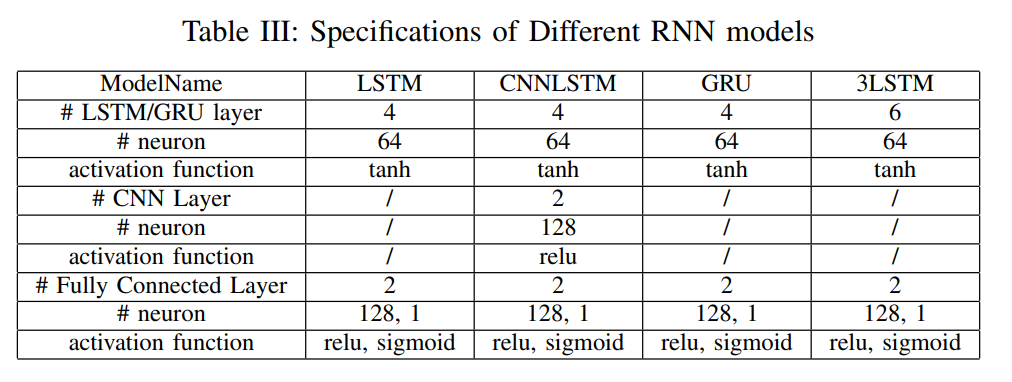
\includegraphics[width=\linewidth]{fig/deep-defense-architecture.png}
	\caption{Kiến trúc các mô hình của DeepDefense \cite{28-Yuan}}
	\label{fig:deep-defense-architecture}
\end{figure}

\textit{Mô hình LUCID}\cite{27-Corin}

Trong nghiên cứu này, tác giả tận dụng sự đơn giản mà hiệu quả của lớp Conv1D và Max  Pooling trong mạng CNN. Để xây dựng dataset, tác giả rút trích 11 đặc trưng của các gói tin và sắp xếp theo trình tự thời gian (time-series) với số lượng n cố định. Với các siêu tham số n (số lượng packet tối đa của 1 mẫu), t (thời gian quan sát tối đa 1 mẫu), k (số kernel của Conv1D), h (số filter của Conv1D), m (kích thước của Max Pooling), tác giả có thể tùy chỉnh các thông số này sao cho thu được mô hình có độ chính xác cao nhất. Cuối cùng với bộ siêu tham số n = 100, t = 100, k = 64, h = 3, m = 98, tác giả thu được độ chính xác mô hình trên dataset ISCX 2012 \cite{35-Shiravi} là 98.88\%. So với mô hình DeepDefense ở trên, mô hình LUCID có độ chính xác cao hơn và  đơn giản hơn nhiều lần. Kiến trúc của mô hình LUCID được thể hiện trong hình \ref{fig:lucid-model}.

\begin{figure}[ht!]
	\centering
	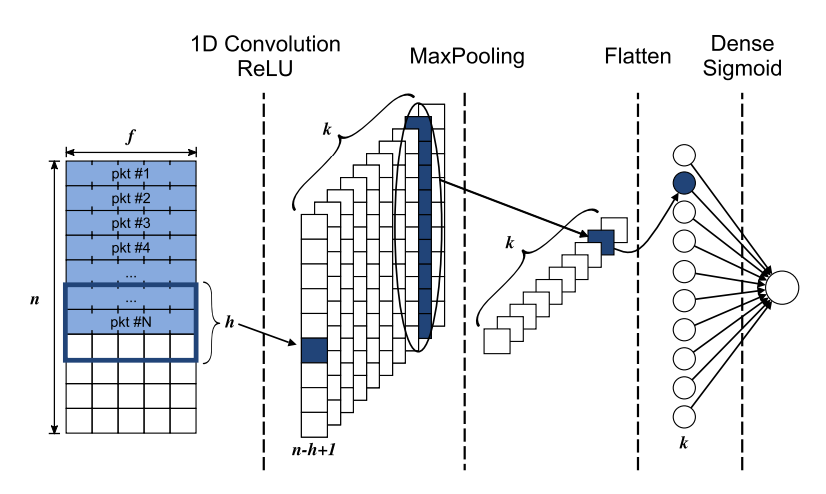
\includegraphics[width=0.6\linewidth]{fig/lucid-model.png}
	\caption{Kiến trúc mô hình của LUCID \cite{27-Corin}}
	\label{fig:lucid-model}
\end{figure}

\subsubsection{Chi tiết mô hình DNN}

Dựa theo nghiên cứu của Ram B. Basnet và các cộng sự \cite{61-Basnet}, mô hình tôi áp dụng được thể hiện trong hình \ref{fig:dnn-model}.

 \begin{figure}[ht!]
 	\centering
	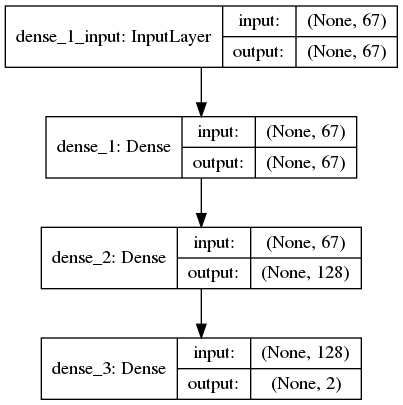
\includegraphics[width=0.5\linewidth]{fig/dnn-model.png}
	\caption{Mô hình học sâu DNN}
	\label{fig:dnn-model}
\end{figure}

Trong đó,

\begin{itemize}
	\item[--] Lớp Input: đầu vào có dạng (67,1) tương ứng với dạng của một bản ghi trong dataset có 67 đặc trưng của một luồng gói tin.
	\item[--] Lớp Dense\_1: lớp này có 67 đơn vị giúp rút trích đặc tính của từng đặc trưng trong dữ liệu. Hàm kích hoạt được dùng là ReLU.
	\item[--] Lớp Dense\_2: lớp này có 128 đơn vị. Hàm kích hoạt được dùng là ReLU.
	\item[--] Lớp Fully conntected (dense 3): lớp này có 2 đơn vị để để phân lớp Benign hay Attack. Hàm kích hoạt được dùng là Softmax.
\end{itemize}

\subsubsection{Huấn luyện mô hình DNN trên tập IDS-train}

Để huấn luyện mô hình, tôi sử dụng hàm tối ưu là Adam \cite{60-Kingma}, hàm mất mát là CategoricalCrossEntropy.

Trước khi huấn luyện, tôi tách tập \textit{IDS-train} thành hai phần là phần huấn luyện và phần xác thực với tỷ lệ 8:2. Sau khi huấn luyện với 10 epoch, tôi thu được kết quả với độ chính xác là 99.59\% trên tập xác thực.

Biểu đồ trong hình \ref{fig:dnn-train-acc} thể hiện độ chính xác và biểu đồ trong hình \ref{fig:dnn-train-loss} thể hiện sự mất mát trong quá trình huấn luyện.

\begin{figure}[!htb]
	\begin{minipage}{0.48\textwidth}
		\centering
		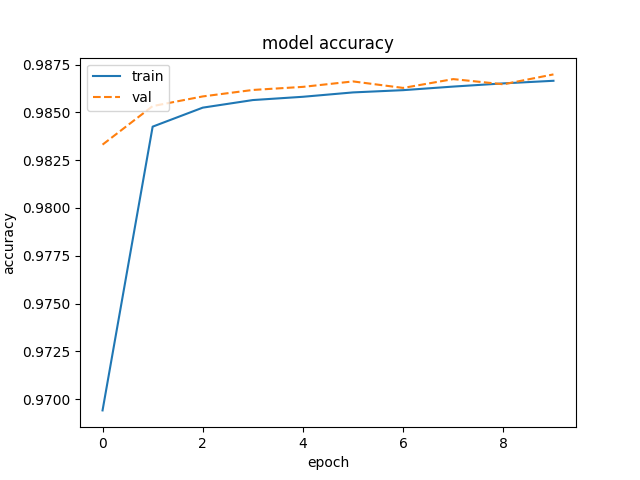
\includegraphics[width=\linewidth]{fig/dnn-train-acc.png}
		\caption{Độ chính xác mô hình DNN trong quá trình huấn luyện}
		\label{fig:dnn-train-acc}
	\end{minipage}\hfill
	\begin{minipage}{0.48\textwidth}
		\centering
		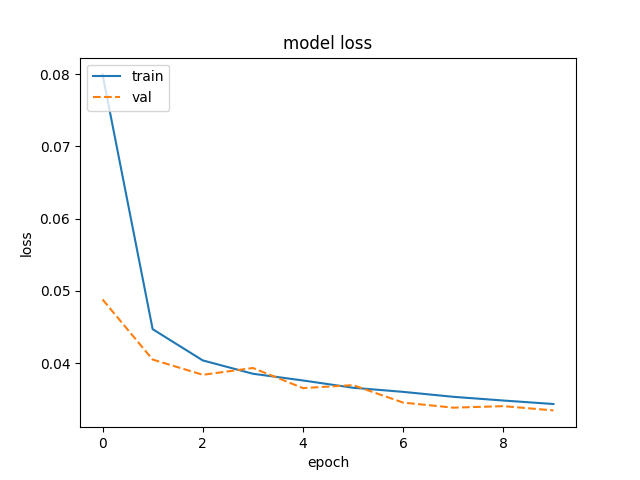
\includegraphics[width=\linewidth]{fig/dnn-train-loss.png}
		\caption{Độ mất mát mô hình DNN trong quá trình huấn luyện}
		\label{fig:dnn-train-loss}
	\end{minipage}
\end{figure}

\subsubsection{Kiểm thử mô hình DNN trên tập IDS-test}

Kiểm thử mô hình đã huấn luyện ở trên, tôi thu được kết quả đạt độ chính xác 99.22\%. Bảng \ref{tab:dnn-confusion-matrix} biểu thị ma trận nhầm lẫn.

\begin{table}[ht!]
	\centering
	\begin{tabular}{|l|l|l|l|}
		\hline
		&                   & \textbf{Predicted} &                   \\ \hline
		&                   & \textit{Negative}  & \textit{Positive} \\ \hline
		\textbf{True} & \textit{Negative} & 1,813,764          & 7,988             \\ \hline
		& \textit{Positive} & 9,291              & 374,356           \\ \hline
	\end{tabular}
\caption{Ma trận nhầm lẫn mô hình DNN trên tập IDS-Test}
\label{tab:dnn-confusion-matrix}
\end{table}

Từ ma trận nhầm lẫn, tôi có được các chỉ số đánh giá mô hình của mình trong bảng \ref{tab:dnn-result}.

\begin{table}[ht!]
	\centering
	\begin{tabular}{|l|l|l|l|l|}
		\hline
		\multicolumn{1}{|c|}{\textbf{Mô hình}} &
		\multicolumn{1}{c|}{\textbf{Accuracy (\%)}} &
		\multicolumn{1}{c|}{\textbf{Precision (\%)}} &
		\multicolumn{1}{c|}{\textbf{Recall (\%)}} &
		\multicolumn{1}{c|}{\textbf{F1-score (\%)}} \\ \hline
		DNN &
		99.22 &
		97.91 &
		97.58 &
		97.74 \\ \hline
	\end{tabular}
\caption{Kết quả mô hình DNN trên tập IDS-test}
\label{tab:dnn-result}
\end{table}

\subsubsection{So sánh kết quả mô hình DNN với DeepDefense và LUCID}

Vì các mô hình DeepDefense \cite{28-Yuan} và LUCID \cite{27-Corin} chưa được tôi cài đặt và kiểm thử trên một tập dữ liệu, vì vậy tôi sẽ so sánh kết quả của mô hình DNN của tôi với các kết quả được công bố trong các nghiên cứu trên. Kết quả so sánh được biểu thị trong bảng \ref{tab:dnn-comparision}.

\begin{table}[ht!]
	\begin{tabular}{|l|l|l|l|l|}
		\hline
		\multicolumn{1}{|c|}{\textbf{Mô hình}} &
		\multicolumn{1}{c|}{\textbf{Accuracy (\%)}} &
		\multicolumn{1}{c|}{\textbf{Precision (\%)}} &
		\multicolumn{1}{c|}{\textbf{Recall (\%)}} &
		\multicolumn{1}{c|}{\textbf{F1-score (\%)}} \\ \hline
		DNN         & \textbf{99.22} & 97.91          & 97.58          & 97.74          \\ \hline
		LUCID       & 98.88 & \textbf{98.27} & \textbf{99.52} & \textbf{98.89} \\ \hline
		DeepDefense & 98.41          & 98.34          & 98.48          & 98.41          \\ \hline
	\end{tabular}
\caption{So sánh kết quả của mô hình DNN với DeepDefense và LUCID}
\label{tab:dnn-comparision}
\end{table}

Từ số liệu trong bảng \ref{tab:dnn-comparision}, tôi nhận thấy, kết quả của các mô hình trên các tập kiểm thử của chính họ đều đạt được kết quả tốt và đạt được state-of-the-art.

\subsection{So sánh đánh giá các mô hình trên tập IDS-test}
\label{compare-multi-models}

Trong phần này, tôi sẽ so sánh các chỉ số đánh giá và thời gian thực thi giữa các mô hình học máy với mô hình học sâu DNN.

\subsubsection{So sánh đánh giá độ chính xác}

\begin{table}[ht!]
	\centering
	\begin{tabular}{|l|l|}
		\hline
		\multicolumn{1}{|c|}{\textbf{Mô hình}} & \multicolumn{1}{c|}{\textbf{Accuracy (\%)}} \\ \hline
		DT   & \textbf{99.97} \\ \hline
		RF   & \textbf{99.83} \\ \hline
		DNN  & 99.22          \\ \hline
		LSVM & 95.67          \\ \hline
		NB   & 67.69          \\ \hline
	\end{tabular}
\caption{So sánh độ chính xác của các mô hình trên tập IDS-Test}
\label{tab:compare}
\end{table}

 \begin{figure}[ht!]
 	\centering
	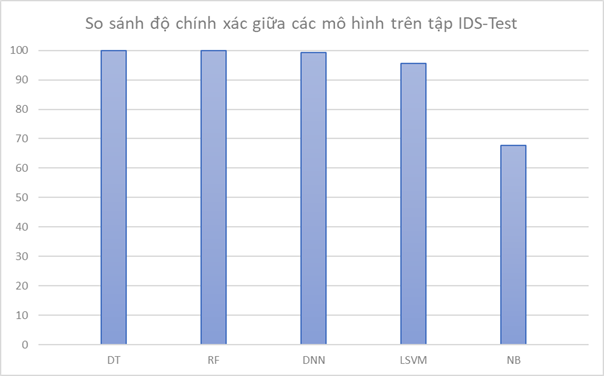
\includegraphics[width=\linewidth]{fig/compare-acc.png}
	\caption{So sánh độ chính xác các mô hình trên tập IDS-test}
	\label{fig:compare-acc}
\end{figure}

Từ bảng \ref{tab:compare} và biểu đồ hình \ref{fig:compare-acc}, có thể thấy, hai mô hình học máy có tiếp cận đơn giản là Decision Tree và Random Forest có độ chính xác cao hơn mô hình DNN. Điều này cho thấy sự đơn giản mà hiệu quả của các mô hình học máy trong việc nhận diện tấn công DoS/DDoS so với mô hình học sâu DNN có kiến trúc phức tạp và đòi hỏi nhiều tài nguyên tính toán hơn.

\subsubsection{So sánh và đánh giá thời gian thực thi}

Trong phần này tôi sẽ đánh giá thời gian thực thi giữa hai mô hình Decision Tree và DNN. Để đánh giá và so sánh thời gian thực thi của hai mô hình, tôi sử dụng phần cứng với CPU Intel Core I7-8700 và bộ nhớ RAM 32GB. Tổng số mẫu trong IDS-Test là 2,205,399 mẫu. Kết quả được biểu thị trong bảng \ref{tab:compare-runtime}.

\begin{table}[ht!]
	\centering
	\begin{tabular}{|l|l|l|}
		\hline
		\multicolumn{1}{|c|}{\textbf{Mô hình}} &
		\multicolumn{1}{c|}{\textbf{\begin{tabular}[c]{@{}c@{}}Thời gian \\ thực thi (giây)\end{tabular}}} &
		\multicolumn{1}{c|}{\textbf{\begin{tabular}[c]{@{}c@{}}Thời gian thực thi\\ trung bình 1 mẫu (giây)\end{tabular}}} \\ \hline
		DT &
		\textbf{0.4} &
		\textbf{$2 \cdot 10^{-7}$} \\ \hline
		DNN &
		8.5 &
		$4 \cdot 10^{-6}$  \\ \hline
	\end{tabular}
\caption{So sánh thời gian thực thi giữa DT và DNN}
\label{tab:compare-runtime}
\end{table}

Từ kết quả trong bảng \ref{tab:compare-runtime}, tôi nhận thấy thời gian thực thi mô hình Decision Tree nhanh hơn đáng kể so với mô hình DNN (gấp 22 lần). Từ đó cho thấy, Decision Tree không những vượt trội hơn DNN về độ chính xác mà còn vượt trội hơn cả về thời gian thực thi.

\section{Phát triển phần mềm phát hiện tấn công DoS/DDoS – IDS-DDoS}

Sau khi huấn luyên các mô hình học máy và học sâu, tôi tiến hành viết phần mềm phát hiện tấn công mạng trong thời gian thực.

\subsection{Kiến trúc của phần mềm}

Ý tưởng của phần mềm là sẽ lắng nghe các gói tin trên một giao diện mạng, khi phát hiện một luồng tấn công, thông báo sẽ được gửi lên một máy chủ thông qua unix socket. Lưu đồ của phần mềm được thể hiện trong hình \ref{fig:ids-software}.

\begin{figure}[ht!]
	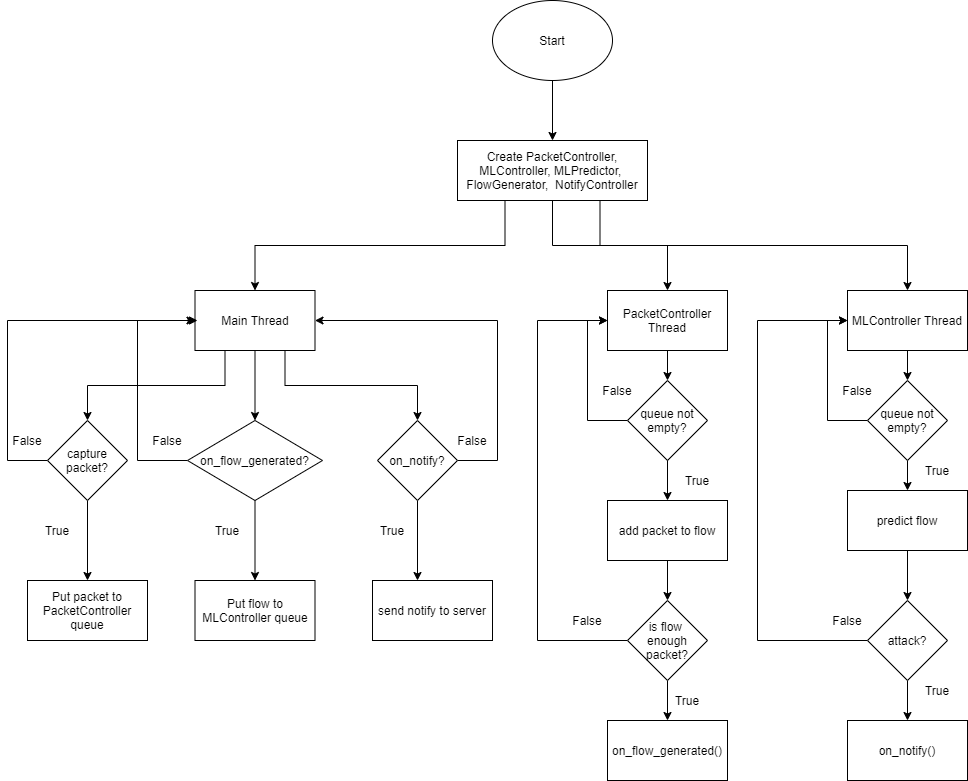
\includegraphics[width=\linewidth]{fig/ids-software.png}
	\caption{Lưu đồ phần mềm IDS-DDoS}
	\label{fig:ids-software}
\end{figure}

Phần mềm được thiết kế chạy đa tiểu trình (multi-thread). Trong đó có 3 tiểu trình là MainThread, PacketControllerThread và MLControllerThread.

\textit{MainThread}

Trong tiểu trình này, các gói tin sẽ được thu thập trên một giao diện mạng (một card mạng), cứ mỗi lần bắt được một gói tin, tiểu trình này sẽ đẩy thông tin gói tin đó vào trong hàng đợi (queue) của PacketControllerThread để chở xử lý tạo ra các luồng gói tin (flow). Bên cạnh đó, tiểu trình này có hai hàm callback là \textbf{on\_flow\_generated} và \textbf{on\_notify}. Mỗi khi PacketControllerThread tạo ra 1 flow mới, nó sẽ gọi hàm \textbf{on\_flow\_generated} để thông báo, khi nhận được thông báo MainThread sẽ đẩy flow này vào trong queue của MLControllerThread để chờ xử lý. Mỗi khi MLControllerThread xử lý xong, nó sẽ gọi hàm \textbf{on\_notify} để thông báo cho MainThread. Hàm \textbf{on\_notify} ở MainThread có chức năng là sẽ đẩy thông điệp đến một socket server thông qua unix socket.

\textit{PacketControllerThread}

Tiểu trình này sẽ có một vòng lặp vô tận kiểm tra xem queue có phần tử không, nếu có nó sẽ tiến hành lấy gói tin trong queue ra, biến đổi thành đối tượng lớp BasicPacketInfo, đối tượng này sẽ được xử lý trong lớp FlowGenerator. FlowGenerator sẽ liên tục đẩy các BasicPacketInfo vào đối tượng lớp BasicFlow cho đến khi nhận được gói tin kết thúc hoặc timeout. Cuối cùng nó sẽ đẩy đối tượng lớp BasicFlow vào hàm \textbf{on\_flow\_generated}.

\textit{MLControllerThread}

Tương tự PacketControllerThread, tiểu trình này cũng có một vòng lặp để kiểm tra queue, nếu có phần tử (flow) nó sẽ tiến hành phân loại flow này, nếu là flow độc hại (tấn công DoS/DDoS) nó sẽ gọi hàm \textbf{on\_notify}.

\subsection{Rút trích các đặc trưng}

Để rút trích đặc trưng của một luồng gói tin, tôi sử dụng 3 lớp là BasicPacketInfo, BasicFlow và FlowGenerator được mô tả như bên dưới. Toàn bộ giải thuật của các lớp này được tôi tham khảo mã nguồn phần mềm CICFlowMeter \cite{37-cicflowmeter}. Lý do là vì dataset mà tôi sử dụng để huấn luyện được tạo ra từ phần mềm này.

\textit{Lớp BasicPacketInfo}

Gói tin mạng có rất nhiều thành phần, vì vậy cần phải phân tích và lấy ra các thông tin thiết yếu. Các thông tin này sẽ được đưa vào lớp BasicPacketInfo. Các thông tin đó gồm: địa chỉ IP nguồn, địa chỉ IP đích, cổng nguồn, cổng đích, giao thức, timestamp, số lượng bytes trong payload, các flag FIN, PSH, URG, ECE, SYN, ACK, CWR, RST, TCP window, số byte trong header.

\textit{Lớp BasicFlow}

Từ thông tin của các BasicPacketInfo, lớp này sẽ tính toán các đặc trưng. Các đặc trưng này được liệt kê trong bảng \ref{tab:feature-list}. Các đặc trưng chủ yếu là các con số thống kê max, min, trung bình, độ lệch chuẩn và phương sai.

\textit{Lớp FlowGenerator}

Lưu đồ của lớp này được thể hiện trong hình \ref{fig:flow-gen}.

\begin{figure}[ht!]
	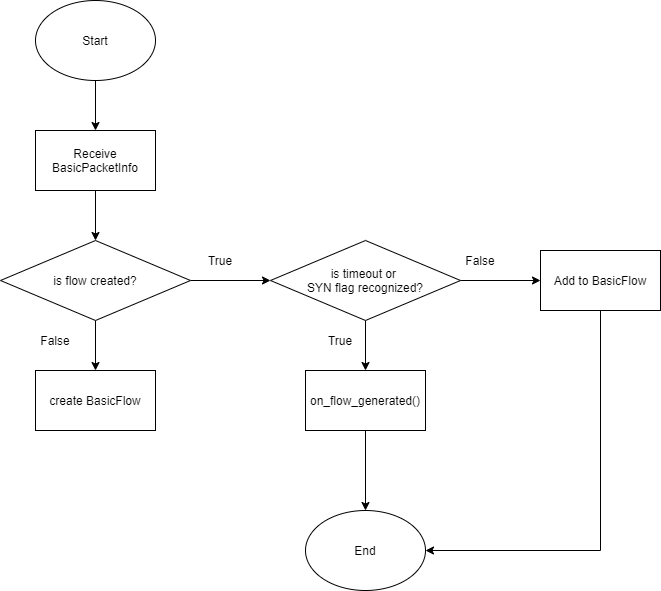
\includegraphics[width=\linewidth]{fig/flow-gen.png}
	\caption{Lưu đồ lớp FlowGenerator}
	\label{fig:flow-gen}
\end{figure}

\subsection{Sử dụng phần mềm}

Phần mềm có giao diện console. Để chạy được cần cung cấp các thông tin gồm giao diện mạng, đường dẫn đến unixsocket server, tên mô hình học máy/học sâu, các đường dẫn đến tệp lưu trữ mô hình.

python3 ids-ddos.py <network interface> <unixsocket path> <model name> <model path>

Ví dụ, lắng nghe trên eth0 và gửi qua socket /tmp/ids-ddos.

DT: \textit{python3 ids-ddos.py eth0 /tmp/ids-ddos svm ./model/dt\_model.pkl}

DNN: \textit{python3 ids-ddos.py eth0 /tmp/ids-ddos svm ./model/dnn-model.json,./model/dnn-weights.hdf5}

\section{Xây dựng SDN controller bằng RYU}
\label{traffic-monitor}

SDN controller của tôi được thiết kế để làm các nhiệm vụ:

\begin{itemize}
	\item[--] Là một switch controller cho các host trong mạng SDN.
	\item[--] Là một traffic monitor các gói tin đi và đến trong mạng, tín hiệu và dữ liệu này được gửi từ Open vSwitch.
	\item[--] Là một unixsocket server nhận tín hiệu từ phần mềm IDS-DDoS.
\end{itemize}

Lưu đồ trong hình \ref{fig:sdn-controller} thể hiện giải thuật của SDN controller, tuy nhiên tôi không thể hiện phần switch controller, vì đây là phần đơn giản được sao chép từ ví dụ của nhà phát triển.

\begin{figure}[ht!]
	\centering
	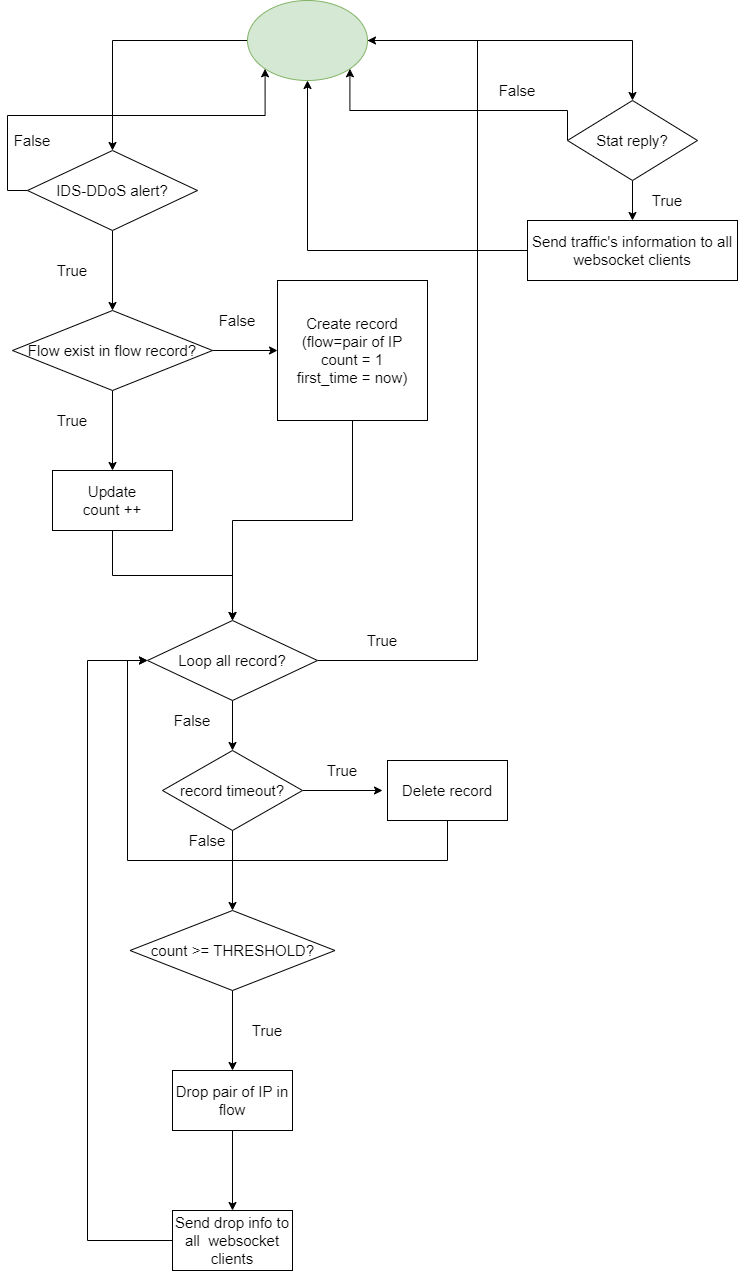
\includegraphics[width=0.75\linewidth]{fig/sdn-controller.png}
	\caption{Lưu đồ của SDN controller}
	\label{fig:sdn-controller}
\end{figure}

SDN controller sẽ tạo ra 2 server

\begin{itemize}
	\item [--] Server unixsocket để chờ tín hiệu từ IDS-DDoS.
	\item [--] Server websocket để gửi tín hiệu đến phần mềm trực quan ở máy khách.
\end{itemize}

Khi nhận được luồng có định dạng là "IP1-IP2" từ IDS-DDoS, trong đó IP1 và IP2 là IP của 2 máy cần phải chặn không cho giao tiếp, controller sẽ tiến hành kiểm tra xem cặp IP này đã được ghi nhận trong bản ghi chưa, nếu chưa thì tạo, nếu có rồi thì cập nhật trạng thái số lượng. Sau đó, controller sẽ tiến hành quét tất cả các luồng trong bản ghi, nếu luồng nào đã timeout (thời gian hiện tại trừ first\_time lớn hơn 1 hằng số giây định trước) thì xóa luồng đó, ngược lại sẽ đi kiểm tra xem luồng tấn công này có được ghi nhận lớn hơn 1 ngưỡng hằng số định trước hay không, nếu có thì chặn luồng này và gửi thông tin này đến tất cả các client đang kết nối vào websocket server, nếu không thì quay lại tiếp tục lắng nghe tín hiệu từ IDS-DDoS.

Tương tự, khi nhận được tín hiệu thống kê lưu lượng từ Open vSwitch, controller sẽ tiến hành broadcast đến tất cả client đang kết nối đến websocket server thông tin này.

Bên cạnh đó, tôi thiết kế một trang web kết nối đến websocket server để trực quan hóa các thông tin chặn luồng, lưu lượng mạng như trình bày ở trên. Hình \ref{fig:webclient-interface} thể hiện giao diện của trang web này.

\begin{figure}[ht!]
	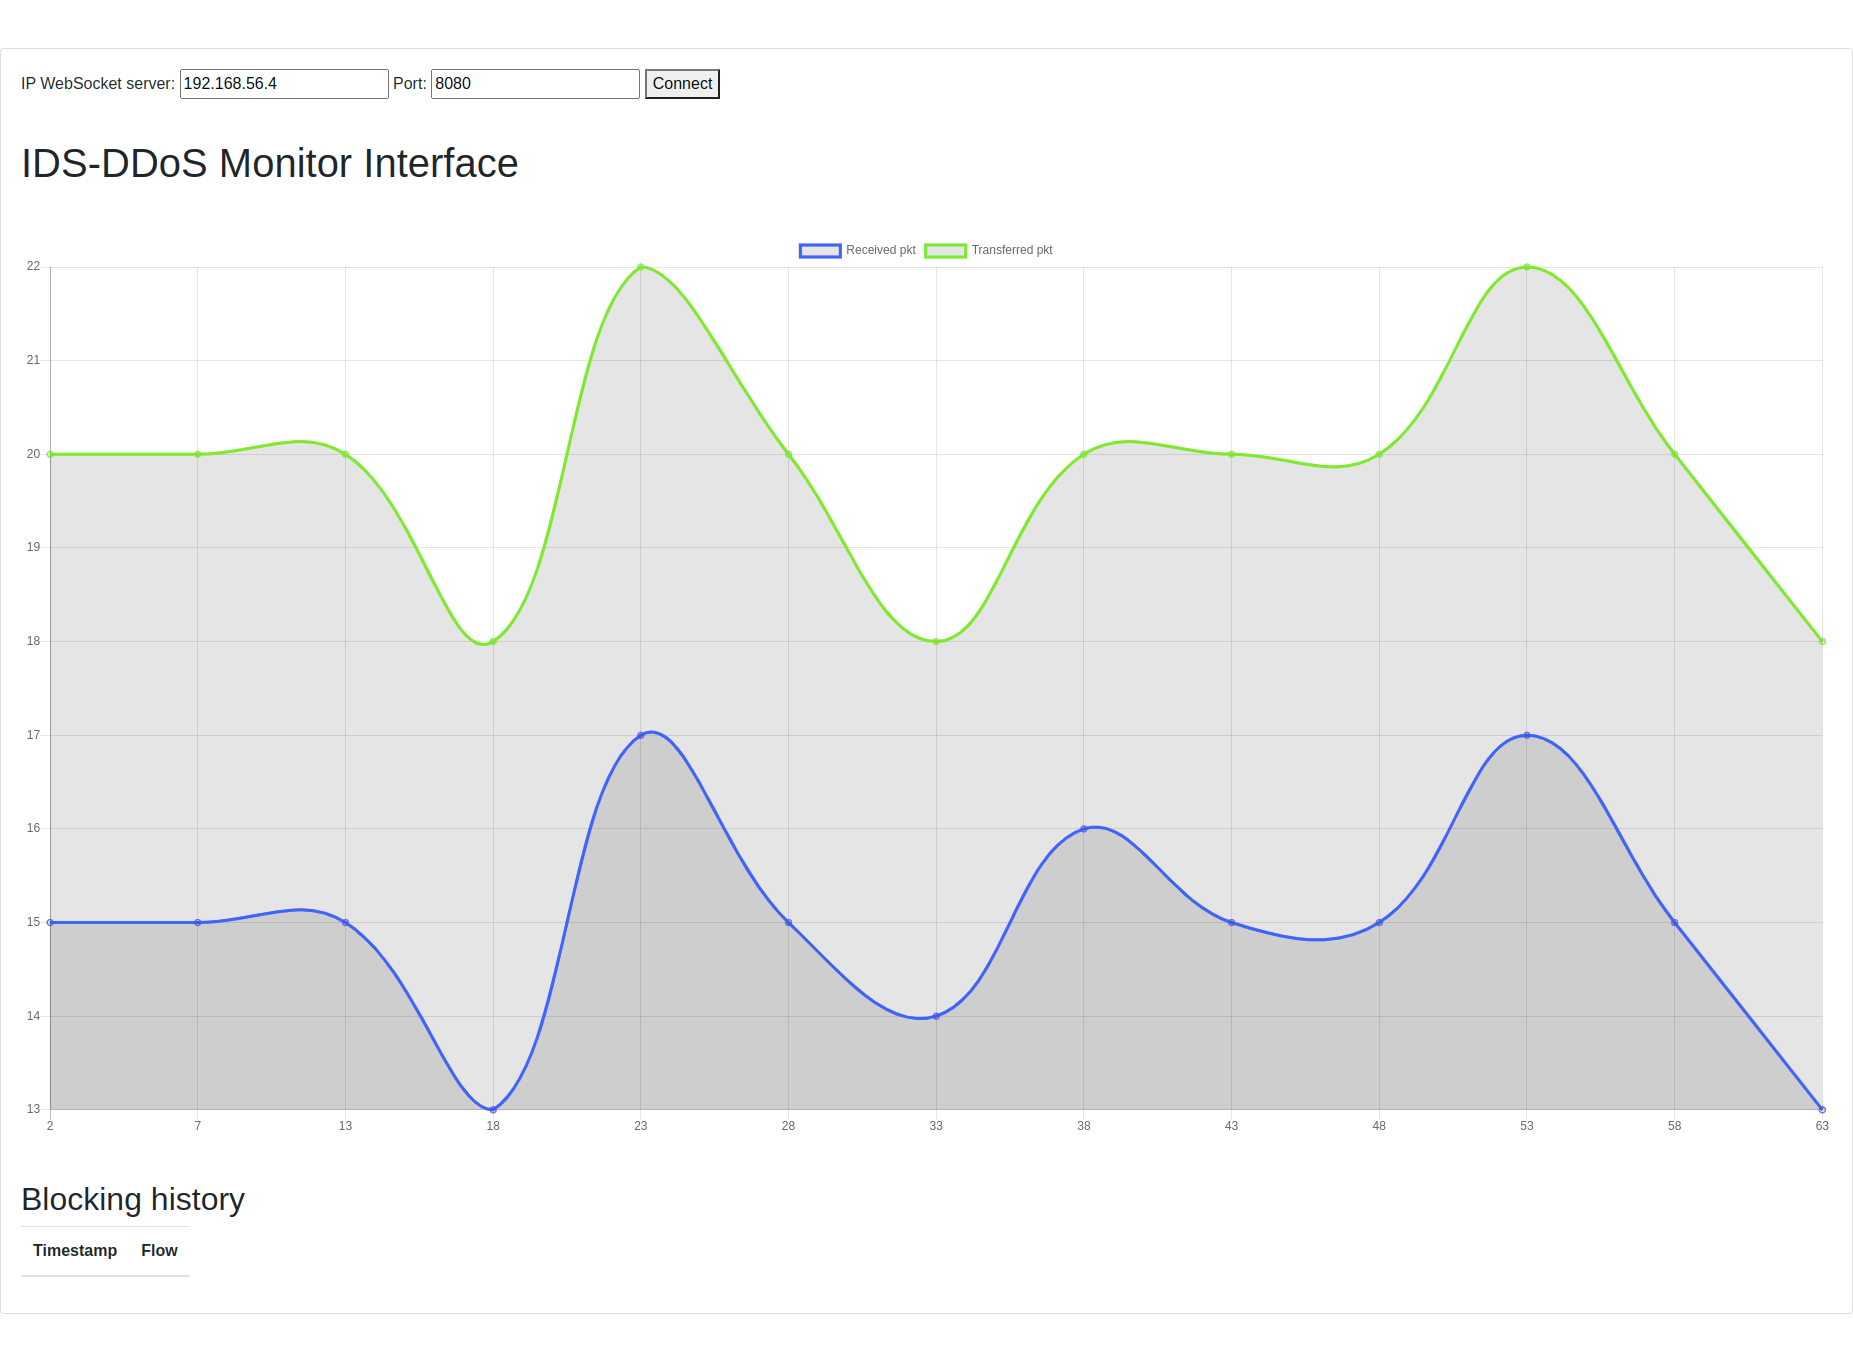
\includegraphics[width=\linewidth]{fig/webclient-interface.png}
	\caption{Giao diện web client thống  kê lưu lượng}
	\label{fig:webclient-interface}
\end{figure}

Trong đó,

\begin{itemize}
	\item [--] Trục tung là số lượng gói tin.
	\item [--] Trục hoành là thời điểm kể từ khi truy cập vào công cụ theo dõi.
	\item [--] Đường màu xanh lá biểu diễn số lượng gói tin được gửi từ trong mạng SDN ra ngoài.
	\item [--] Đường màu xanh dương biểu diễn số lượng gói tin mạng SDN nhận từ bên ngoài.
	\item [--] Bảng "Blocking history" ghi lại các cặp IP đã chặn.
\end{itemize}